\begin{enumerate}

\item 
\begin{enumerate}
	\item The PDE can now be written as
	\[
		\frac{\partial T}{\partial \tau} = -\frac{\beta}{\rho} \left[ \frac{\partial^2 T}{\partial x^2} + \frac{\partial^2 T}{\partial y^2} + \frac{\partial^2 T}{\partial z^2} \right],
	\]
	so we can evaluate the units on both sides:
	\[
	\frac{\Theta}{T} = \frac{[\beta]L^3}{M} \frac{\Theta}{L^2}
	\]
	So we conclude that the units of $\beta$ are $\frac{M}{LT}$.
	
	\item The relevant variables and dimensions are:
	\begin{itemize}
		\item $\tau = $ cooking time ($T$)
		\item $m = $ turkey mass ($M$)
		\item $V = $ turkey volume ($L^3$)
		\item $\beta = $ thermal diffusivity ($M L^{-1} T^{-1}$)
	\end{itemize}


\item The dimensional matrix is
\[ \mathcal{D} = \begin{bmatrix}
 0	& 1	& 0	& 1	 \\
 0	& 0	& 3	& -1 \\
 1	& 0	& 0	& -1
 \end{bmatrix}
\]

It has rank 3 and so the nullity is 1.

\item We find the null space by solving $\mathcal{D} \vec{v} = \vec{0}$:
\[
\begin{cases}
b+ d = 0\\
3c - d = 0 \\
a - d = 0
\end{cases}
\Rightarrow
\begin{cases}
b = -d  \\
3c = d \\
a = d
\end{cases}
\Rightarrow
\begin{bmatrix}
	1 \\ -1 \\ 1/3 \\ 1
\end{bmatrix}
\]
This vector forms a basis of the null space.

\item So Buckingham Pi Theorem states that
\[ 
f(\tau m^{-1} V^{1/3} \beta) = 0 
	\quad \Rightarrow\quad  \tau m^{-1} V^{1/3} \beta = C
	\quad \Rightarrow\quad  \tau = C m V^{-1/3} \beta^{-1}
\]

\item[(f)] Option \#1.

\begin{itemize}
	\item $m_1=2$ implies $\tau_1 = 2$, so $ 1 = C V_1^{-1/3} \beta^{-1}$.
	\item This means that when $m_2=16$, then the mass density remains the same: $\rho = 2/V_1 = 16/V_2$, so $V_2 = 8 V_1$
	\item This means that we should have $\displaystyle\tau_2 = 16 C  V_2^{-1/3} \beta^{-1} =  16 (\Delta V)^{-1/3} \underbrace{C V_1^{-1/3} \beta^{-1}}_{=1} = 16 \cdot 8^{-1/3} \cdot 1$, which implies $\tau = 8$ h.
\end{itemize}

\item[(f)] Option \#2.

First, because the mass density remains the same, we have $\rho = 2/V_1 = 16/V_2$, so $\Delta V = \frac{V_2}{V_1} = 8$.

Then, we have $\tau \propto m V^{-1/3}$, so if the mass is 8 times larger $\Delta m = \frac{m_2}{m_1} = 8$, then $\Delta \tau = \Delta m \cdot \Delta V^{-1/3} = 4$, which means that $\tau$ should be 4 times larger, or 8h.



\end{enumerate}

%
%	\item The relevant variables and dimensions are:
%	\begin{itemize}
%		\item $\tau = $ cooking time ($T$)
%		\item $m = $ turkey mass ($M$)
%		\item $V = $ turkey volume ($L^3$)
%		\item $k = $ thermal conductivity ($MLT^{-3} \Theta^{-1}$)
%		\item $c = $ specific heat ($L^2T^{-2} \Theta^{-1}$)
%	\end{itemize}
%
%
%\item The dimensional matrix is
%\[ \mathcal{D} = \begin{bmatrix}
% 0	& 1	& 0	& 1		& 0 \\
% 0	& 0	& 3	& 1		& 2 \\
% 1	& 0	& 0	& -3	& -2 \\
% 0	& 0	& 0	& -1	& -1
% \end{bmatrix}
%\]
%
%It has rank 4 and so the nullity is 1.
%%
%%\begin{itemize}
%%	\item Rank(D) = 4
%%	\item Nullity = 1
%%\end{itemize}
%
%\item We find the null space by solving $\mathcal{D} \vec{v} = \vec{0}$:
%\[
%\begin{cases}
%b+ d = 0\\
%3c + d + 2e = 0 \\
%a + -3d-2e = 0	 \\
%-d-e=0
%\end{cases}
%\Rightarrow
%\begin{cases}
%b = -3c  \\
%d = 3c \\
%a = 3c\\
%e =  -3c
%\end{cases}
%\Rightarrow
%\begin{bmatrix}
%	3 \\ -3 \\ 1 \\ 3 \\ -3
%\end{bmatrix}
%\]
%This vector forms a basis of the null space.
%
%\item So Buckingham Pi Theorem states that
%\[ 
%f(\tau^3 m^{-3} V k^{3} c^{-3}) = 0 
%	\quad \Rightarrow\quad  \tau^3 m^{-3} V k^{3} c^{-3} = A
%	\quad \Rightarrow\quad  \tau = B m V^{-1/3} c k^{-1}
%\]
%
%\item[(e)] Option \#1.
%
%\begin{itemize}
%	\item $m_1=2$ implies $\tau_1 = 2$, so $ 2 = B V_1^{-1/3} c/k$.
%	\item This means that when $m_2=16$, then the mass density remains the same: $\rho = 2/V_1 = 16/V_2$, so $V_2 = 8 V_1$
%	\item This means that we should have $\tau_2 = 16 B  V_2^{-1/3} c/k =  16 \left(\frac{V_2}{V_1}\right)^{-1/3} B V_1^{-1/3} c/k = 16 \cdot 8^{-1/3} \cdot 2$, which implies $\tau = 8$ h.
%\end{itemize}
%
%\item[(e)] Option \#2.
%
%First, because the mass density remains the same, we have $\rho = 2/V_1 = 16/V_2$, so $\Delta V = \frac{V_2}{V_1} = 8$.
%
%Then, we have $\tau \propto m V^{-1/3}$, so if the mass is 8 times larger $\Delta m = \frac{m_2}{m_1} = 8$, then $\Delta \tau = \Delta m \cdot \Delta V^{-1/3} = 4$, which means that $\tau$ should be 4 times larger, or 8h.
%




\newpage


\item 
\begin{enumerate}

	\item We use the variables in the order given: $v, \rho, E$ to create the dimensional matrix
	\[ \mathcal{D} = 
	\begin{bmatrix}
		0	& 1		& 1 		\\
		1	& -3	& -1 	\\
		-1	& 0		& -2
	\end{bmatrix}
	\]
	
	To find the rank, we transform it into its row echelon form, by first swapping the first two rows:
	\[
	\begin{bmatrix}
		1	& -3	& -1 	\\
		0	& 1		& 1 		\\
		-1	& 0		& -2
	\end{bmatrix}
	\quad \substack{\longrightarrow \\ R_3: R_3+R_1} \quad
		\begin{bmatrix}
			1	& -3	& -1 	\\
			0	& 1		& 1 		\\
			0	& -3		& -3
		\end{bmatrix}
	\quad \substack{\longrightarrow \\ R_3: R_3+3R_2} \quad
		\begin{bmatrix}
			1	& -3	& -1 	\\
			0	& 1		& 1 		\\
			0	& 0		& 0
		\end{bmatrix}
	\]
	
	We conclude that it has rank 2, which means that its nullity is 1.
	
	We find the basis of its vector space:
	\[
	\begin{cases}
		b+c = 0 \\
		a-3b-c=0 \\
		-a-2c = 0
	\end{cases}
	\quad \Rightarrow \quad
		\begin{cases}
			b = -c \\
			\textcolor{gray}{a-3b= c} \\
			a = -2c
		\end{cases}
	\quad \Rightarrow \quad
		\begin{bmatrix}
			2\\ 1 \\ -1
		\end{bmatrix}
	\]
	
	Then the Buckingham Pi Theorem states that 
	\[
	v^2 \rho E^{-1} = m
	\]
	for some constant $m$.
	
	
	\item The previous relationship implies 
	\[ v^2 = m \cdot \left( \frac{E}{\rho} \right) \]
	so in the graph shown, the values should orient themselves along $y = mx$, a line through the origin with slope $m$.
	
	\begin{minipage}{.5\textwidth}
	We can use the data to estimate $m$:
	\[
	m \approx \frac{3\cdot 10^{10}-0}{3\cdot 10^{10}-0} = 1
	\]
	
	so we get 
	\[ v^2 = \frac{E}{\rho}. \]
	\end{minipage}
	\hfill 
	\begin{minipage}{200pt}
		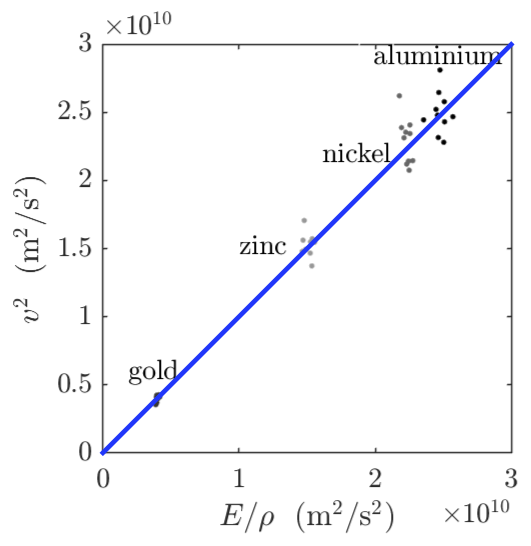
\includegraphics[width=\textwidth]{WaveSpeed_YoungModulus-line.png}
	\end{minipage}
\end{enumerate}


\newpage

\item The trick is to consider the correct variables. It is gravity that makes the wave move, so we need to consider it:
\begin{itemize}
	\item $v = $ wave speed ($L T^{-1}$)
	\item $\lambda = $ wavelength ($L$)
	\item $g = $ gravitational acceleration ($L T^{-2}$) 
\end{itemize}

\textit{Note: Usually, when we consider $g$, we also consider mass or mass density since they are related. One of these terms can also be included here, but they will be ``discarded'' by the null space. You should try it to see it for yourself.}

Then the dimensional matrix is
\[
\mathcal{D} = \begin{bmatrix}
 1	& 1		& 1 \\
 -1	& 0		& -2
 \end{bmatrix}
 \]
 which has rank 2 and so nullity 1 with a basis for the null space
 \[
 \begin{bmatrix}
 -2 \\ 1 \\ 1
 \end{bmatrix}
\]


So we obtain the relation $\dfrac{\lambda g}{v^2} = A$ which implies that $v = B \sqrt{\lambda g}$

So if the wavelength is doubles, then the speed is multiplied by a factor of $\sqrt{2}$.
\end{enumerate}
	
